\chapter{RNA editingサイトに関する検出手法の性能評価}

\section{研究背景}
RNA編集は、転写物の塩基配列を変化させる転写後修飾であり、高等真核生物ではADARによるアデニンからイノシンへのA-to-I編集が最もよく知られる。近年、ゲノムワイドなA-to-I編集サイトの研究から、ヒトでは数千の編集サイトが同定されたと報告されている。RNA編集サイトはゲノムと転写物の一塩基ミスマッチとして検出されるが、シーケンシングやマッピングに起因した擬陽性を多く含む。そのため、真の編集サイトとエラーに起因した擬陽性を高精度に分離させる検出手法がこれまで多く開発されてきたが、開発された手法における検出精度の定量的なベンチマークは行われていない。そこで本研究は、ヒト・マウス・ショウジョウバエのRNA-seqデータを用いた既存の検出手法のベンチマークを行った。ベンチマーキングには、再現率/適合率といった指標を導入することにより、各手法の検出能の定量的な比較を行った。その結果、シーケンシング手法など実験デザイン及び検出手法ごとの特徴を明らかにした。この結果を交えながら、どのような検出パラメータがRNA編集サイトの高精度な検出に寄与するのかについて議論したい。

\section{対象と手法}
\subsection{性能評価に用いた指標}
これまでに開発されてきたRNA editingサイトの検出手法を統一的な指標によって性能評価を行うため、適合率 (Precision)・再現率 (Recall)・F値 (F-measure)と呼ばれる3つの指標を導入した。以下にぞれぞれの指標とその計算方法について示した。この3つの手法は、検出精度を評価する互いに異なる指標であり、算出される値が高いほど高精度であることを表す。尚、真のeditingサイトとは、過去に報告例のある既知のeditngサイトの集合を意味する。
\par
適合率は、式\ref{eq:precision}に定義され、検出された候補のeditingサイトと真のeditingサイトとの積集合おける候補editingサイトの割合として計算される。適合率は、検出したeditingサイトの候補となった集合に正解が含まれる割合と言うこともできる。
\begin{equation}
	precision = \frac{TP}{TP+FP}
	\label{eq:precision}
\end{equation}
\par
再現率は、式\ref{eq:recall}に定義され、検出された候補サイトが正解セットにエンリッチする割合を示す。
\begin{equation}
	recall = \frac{TP}{TP+FN}
	\label{eq:recall}
\end{equation}
\par
F値は、適合率および再現率の調和平均として式\ref{eq:f_measure}のように定義される。
\begin{equation}
	Fmeasure = 2 \times \frac{precision \times recall}{precision + recall}
	\label{eq:f_measure}
\end{equation}

\subsection{正解セットの構築}
\begin{table}[htbp]
	\begin{center}
		\begin{tabular}{llll}
			\bf{Species} & \bf{Reference genome} & \bf{Studies} & \bf{Collected sites} \\
			\it{H. sapiens} & hg19 & 20 & 333,216 \\
			\it{H. sapiens} & hg18 & 22 & 259,705 \\
			\it{M. musclus} & mm10 & 4 & 8,341 \\
			\it{M. musclus} & mm9 & 4 & 8,352 \\
			\it{D. melanogaster} & dm3 & 3 & 1,969
		\end{tabular}
		\label{tab:collection}
		\caption{収集した生物種毎の正解セット}
	\end{center}
\end{table}

\subsection{精度検証に用いた手法}
\begin{table}[htbp]
	\begin{center}
		\begin{tabular}{lll}
			\bf{Study} & \bf{Samples (tissues/cell lines)} & \bf{Identified sites} \\
			\bi{H. sapiens} \\
			Ramaswami, \it{et al.,} 2012 & GM12878                                               & 74,166 \\
			Ramaswami, \it{et al.,} 2013 & lymphocyte cell lines                                 & 230,402 \\
			Peng, \it{et al.,}      2012 & lymphoblastoid cell line in Han Chinese individual    & 22,696 \\
			Park, \it{et al.,}      2013 & 14 human cell lines (ENCODE project)                  & 13,821 \\
			Zhu, \it{et al.,}       2013 & 16 human tissues, 2 cell lines (Illumina BodyMap 2.0) & 2,246 \\
			Bahn, \it{et al.,}      2012 & U87MG (glioblastoma cell line)                        & 12,791 \\
			\bi{M. musculs} \\
			Gu, \it{et al.,} 2012         & White adipose, Femurs, liver      & 244 \\
			Dillman, \it{et al.,} 2013    & Cerebral cortex, 4 embryonic mice & 177 \\
			Lagarrigue, \it{et al.,} 2013 & Liver, Adipose                    & 363 \\
			\bi{M. melanogaster} \\
			Rodriguez, \it{et al.,} 2012 & Fly head & 1,351 \\
			Graveley, \it{et al.,} 2011  & Fly head & 973 \\
			Ramaswami, \it{et al.,} 2013 & Fly head & 850 \\
		\end{tabular}
		\label{tab:methods}
		\caption{性能評価に用いた手法のリスト}
	\end{center}
\end{table}


\section{既存の手法のベンチマークテスト結果}
\subsection{ヒトのデータセット}
\begin{figure}[htbp]
	\begin{center}
		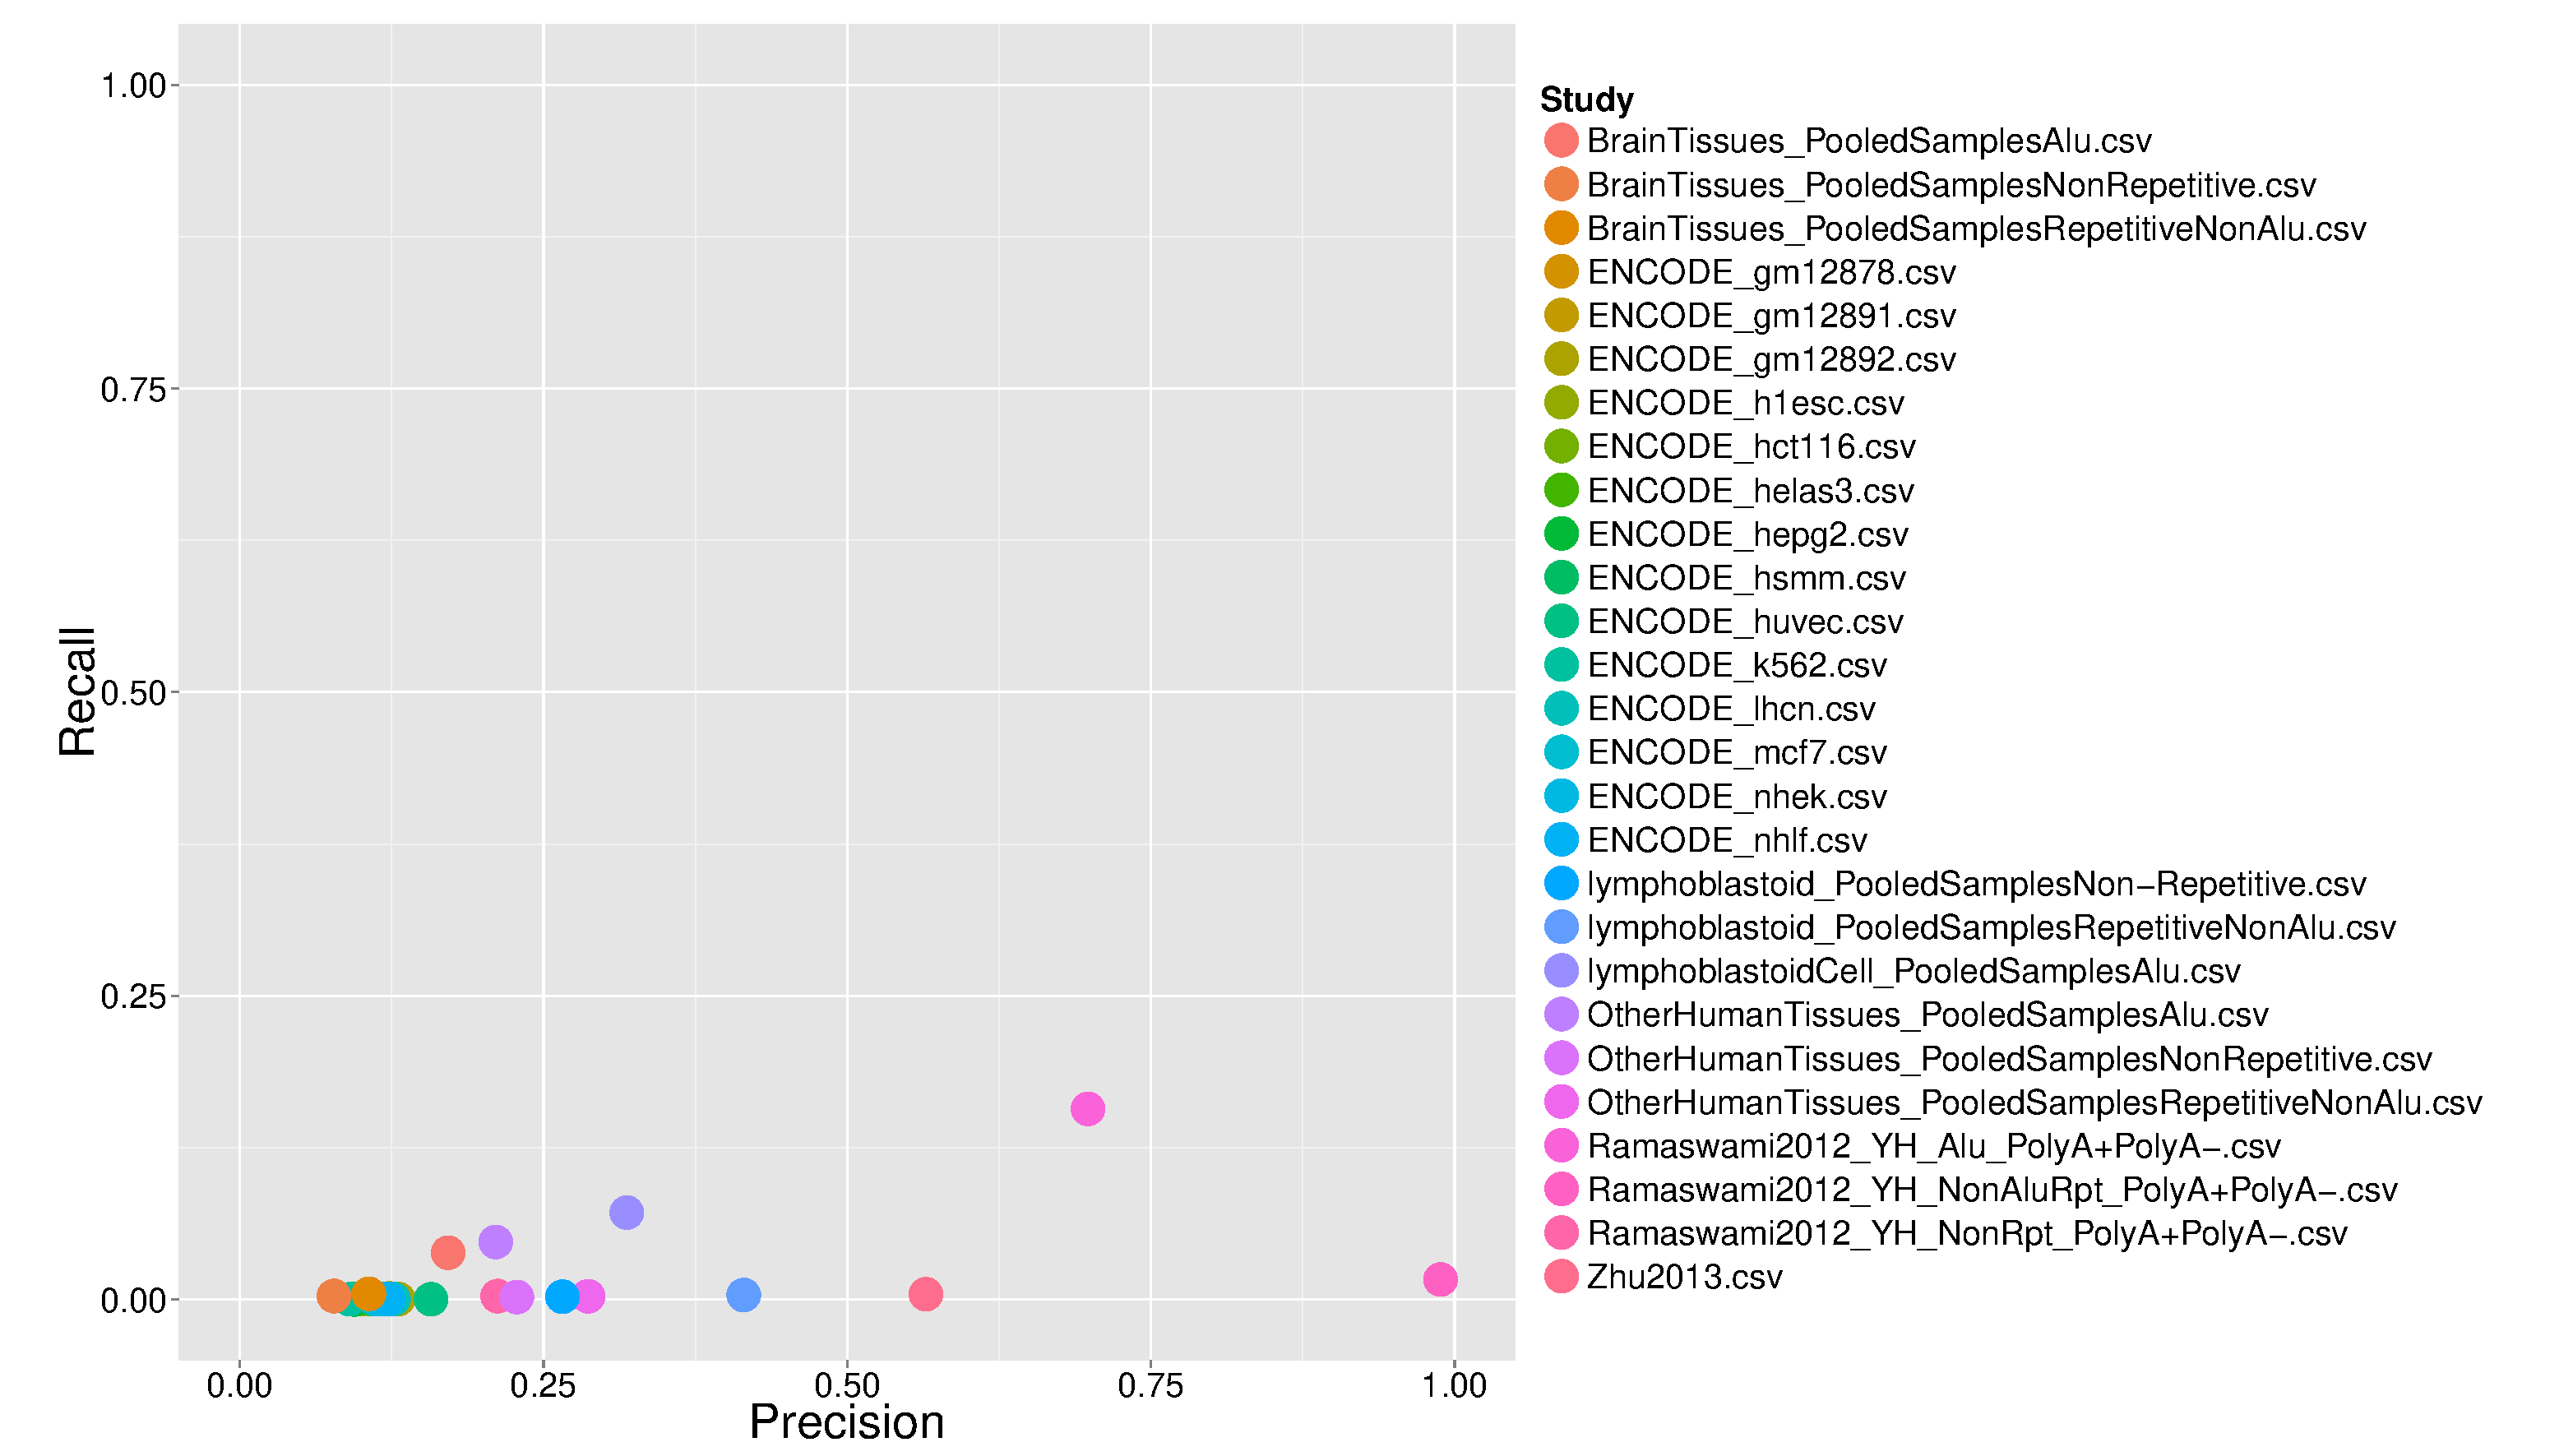
\includegraphics[width=14cm]{bench_human.pdf}
	\end{center}
	\caption{ヒトのデータセットにおける適合率および再現率}
	\label{fig:human_pr}
\end{figure}

\subsection{マウスのデータセット}
\begin{figure}[htbp]
	\begin{center}
		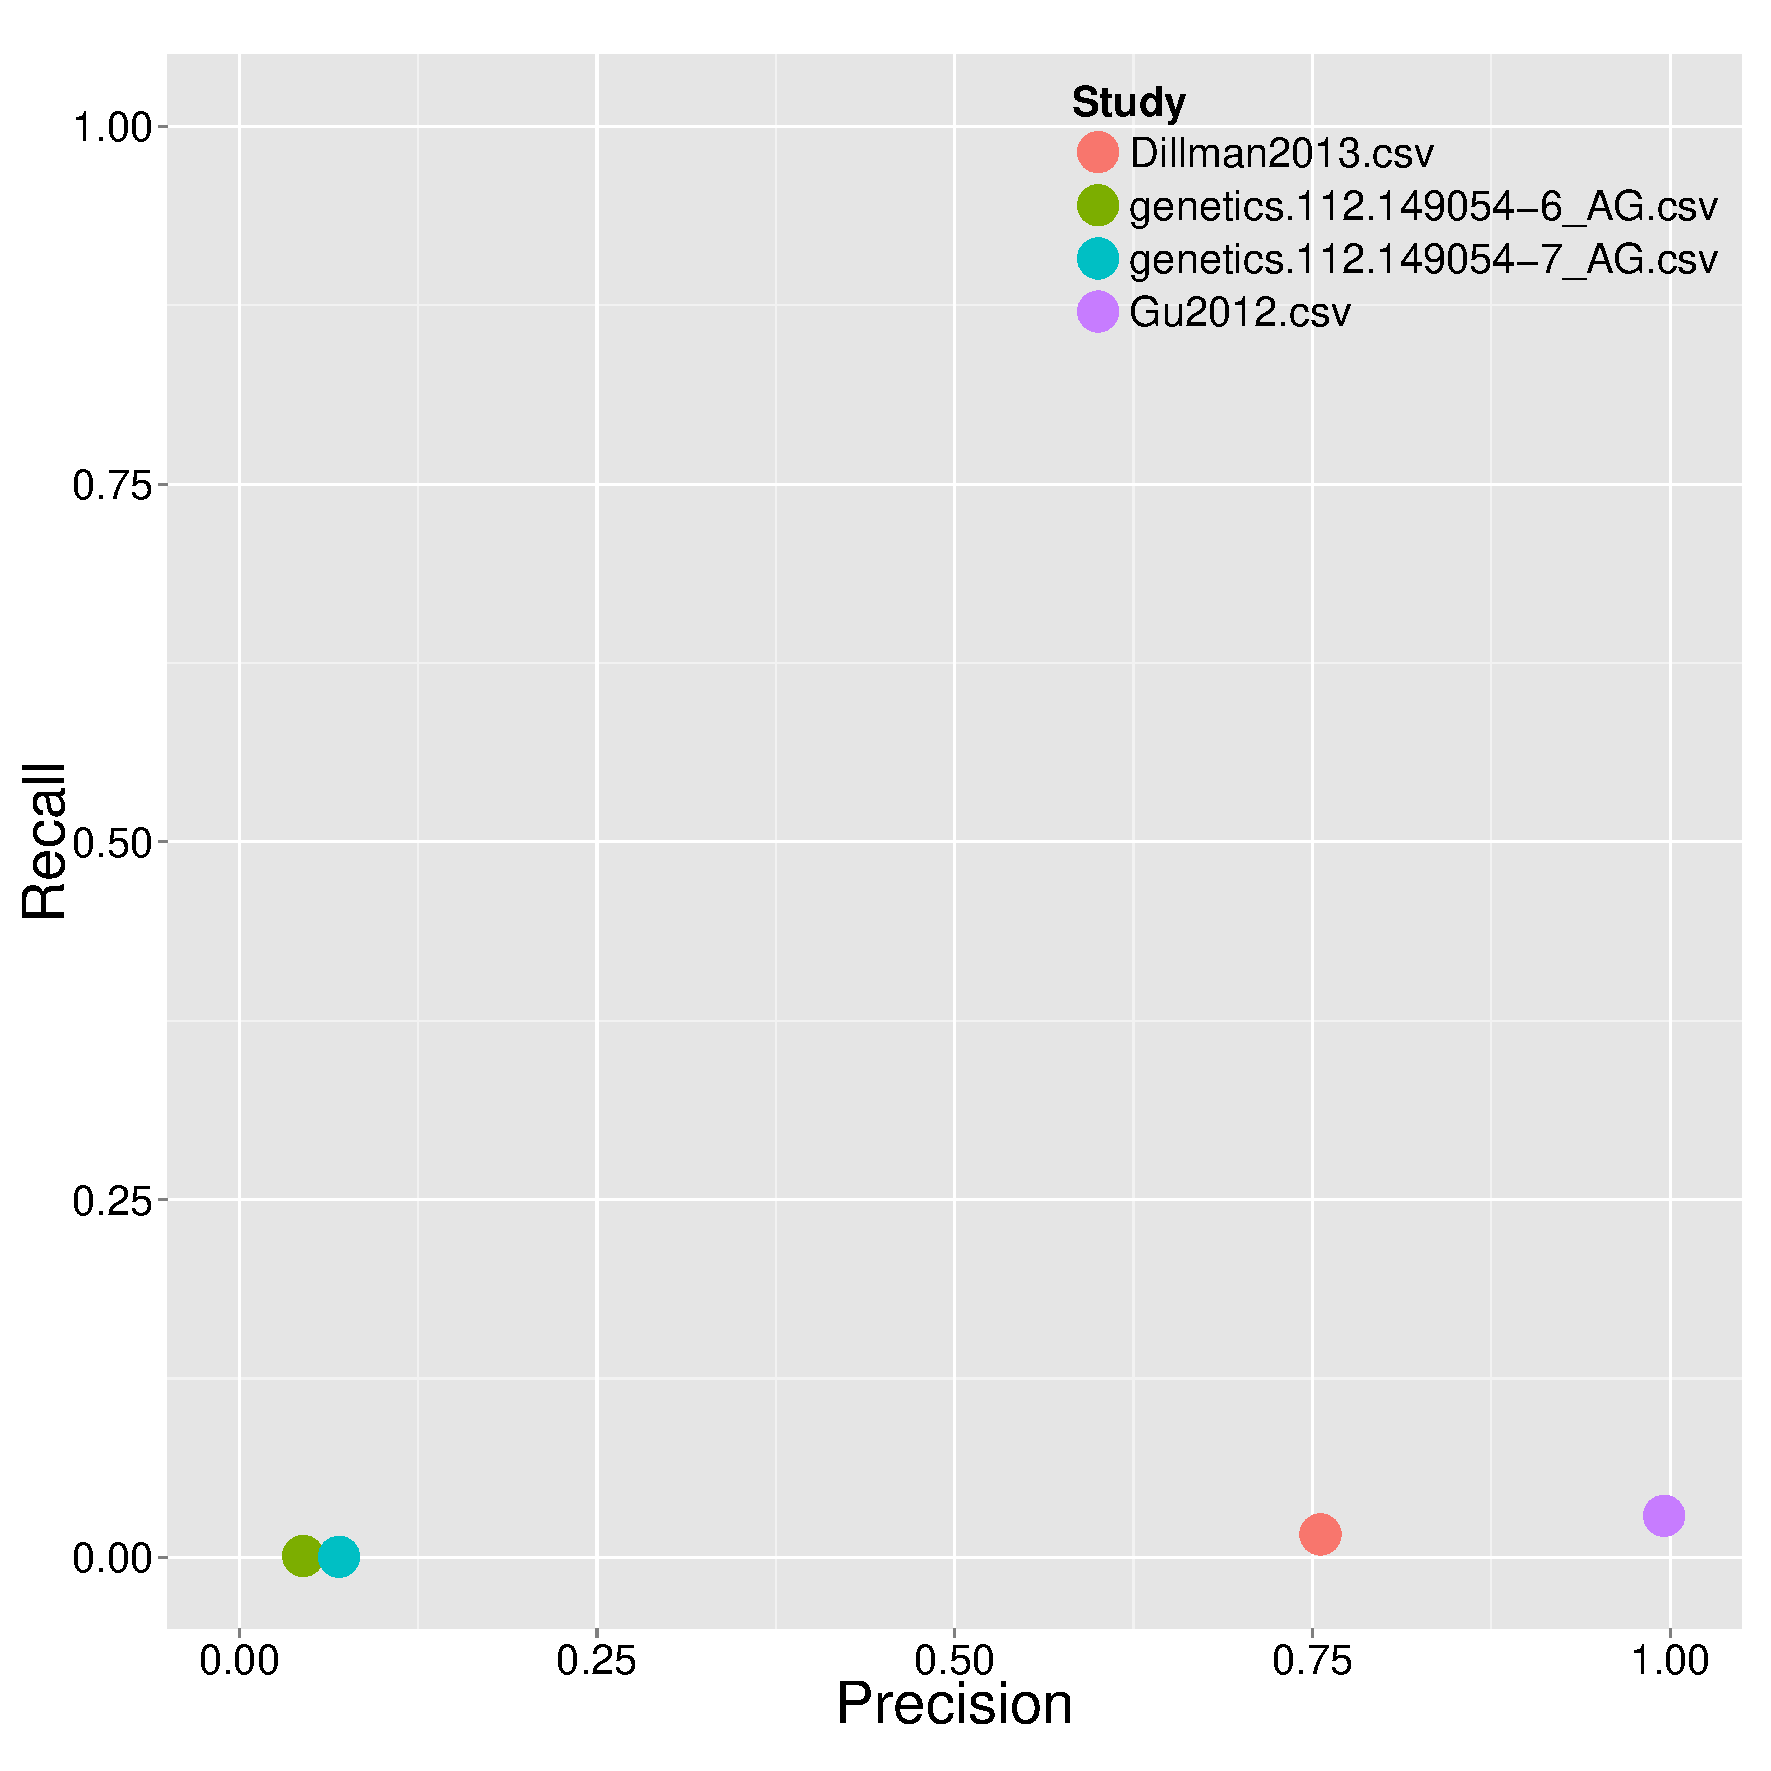
\includegraphics[width=14cm]{bench_mouse.pdf}
	\end{center}
	\caption{マウスのデータセットにおける適合率および再現率}
	\label{fig:mouse_pr}
\end{figure}

\subsection{ショウジョウバエのデータセット}
\begin{figure}[htbp]
	\begin{center}
		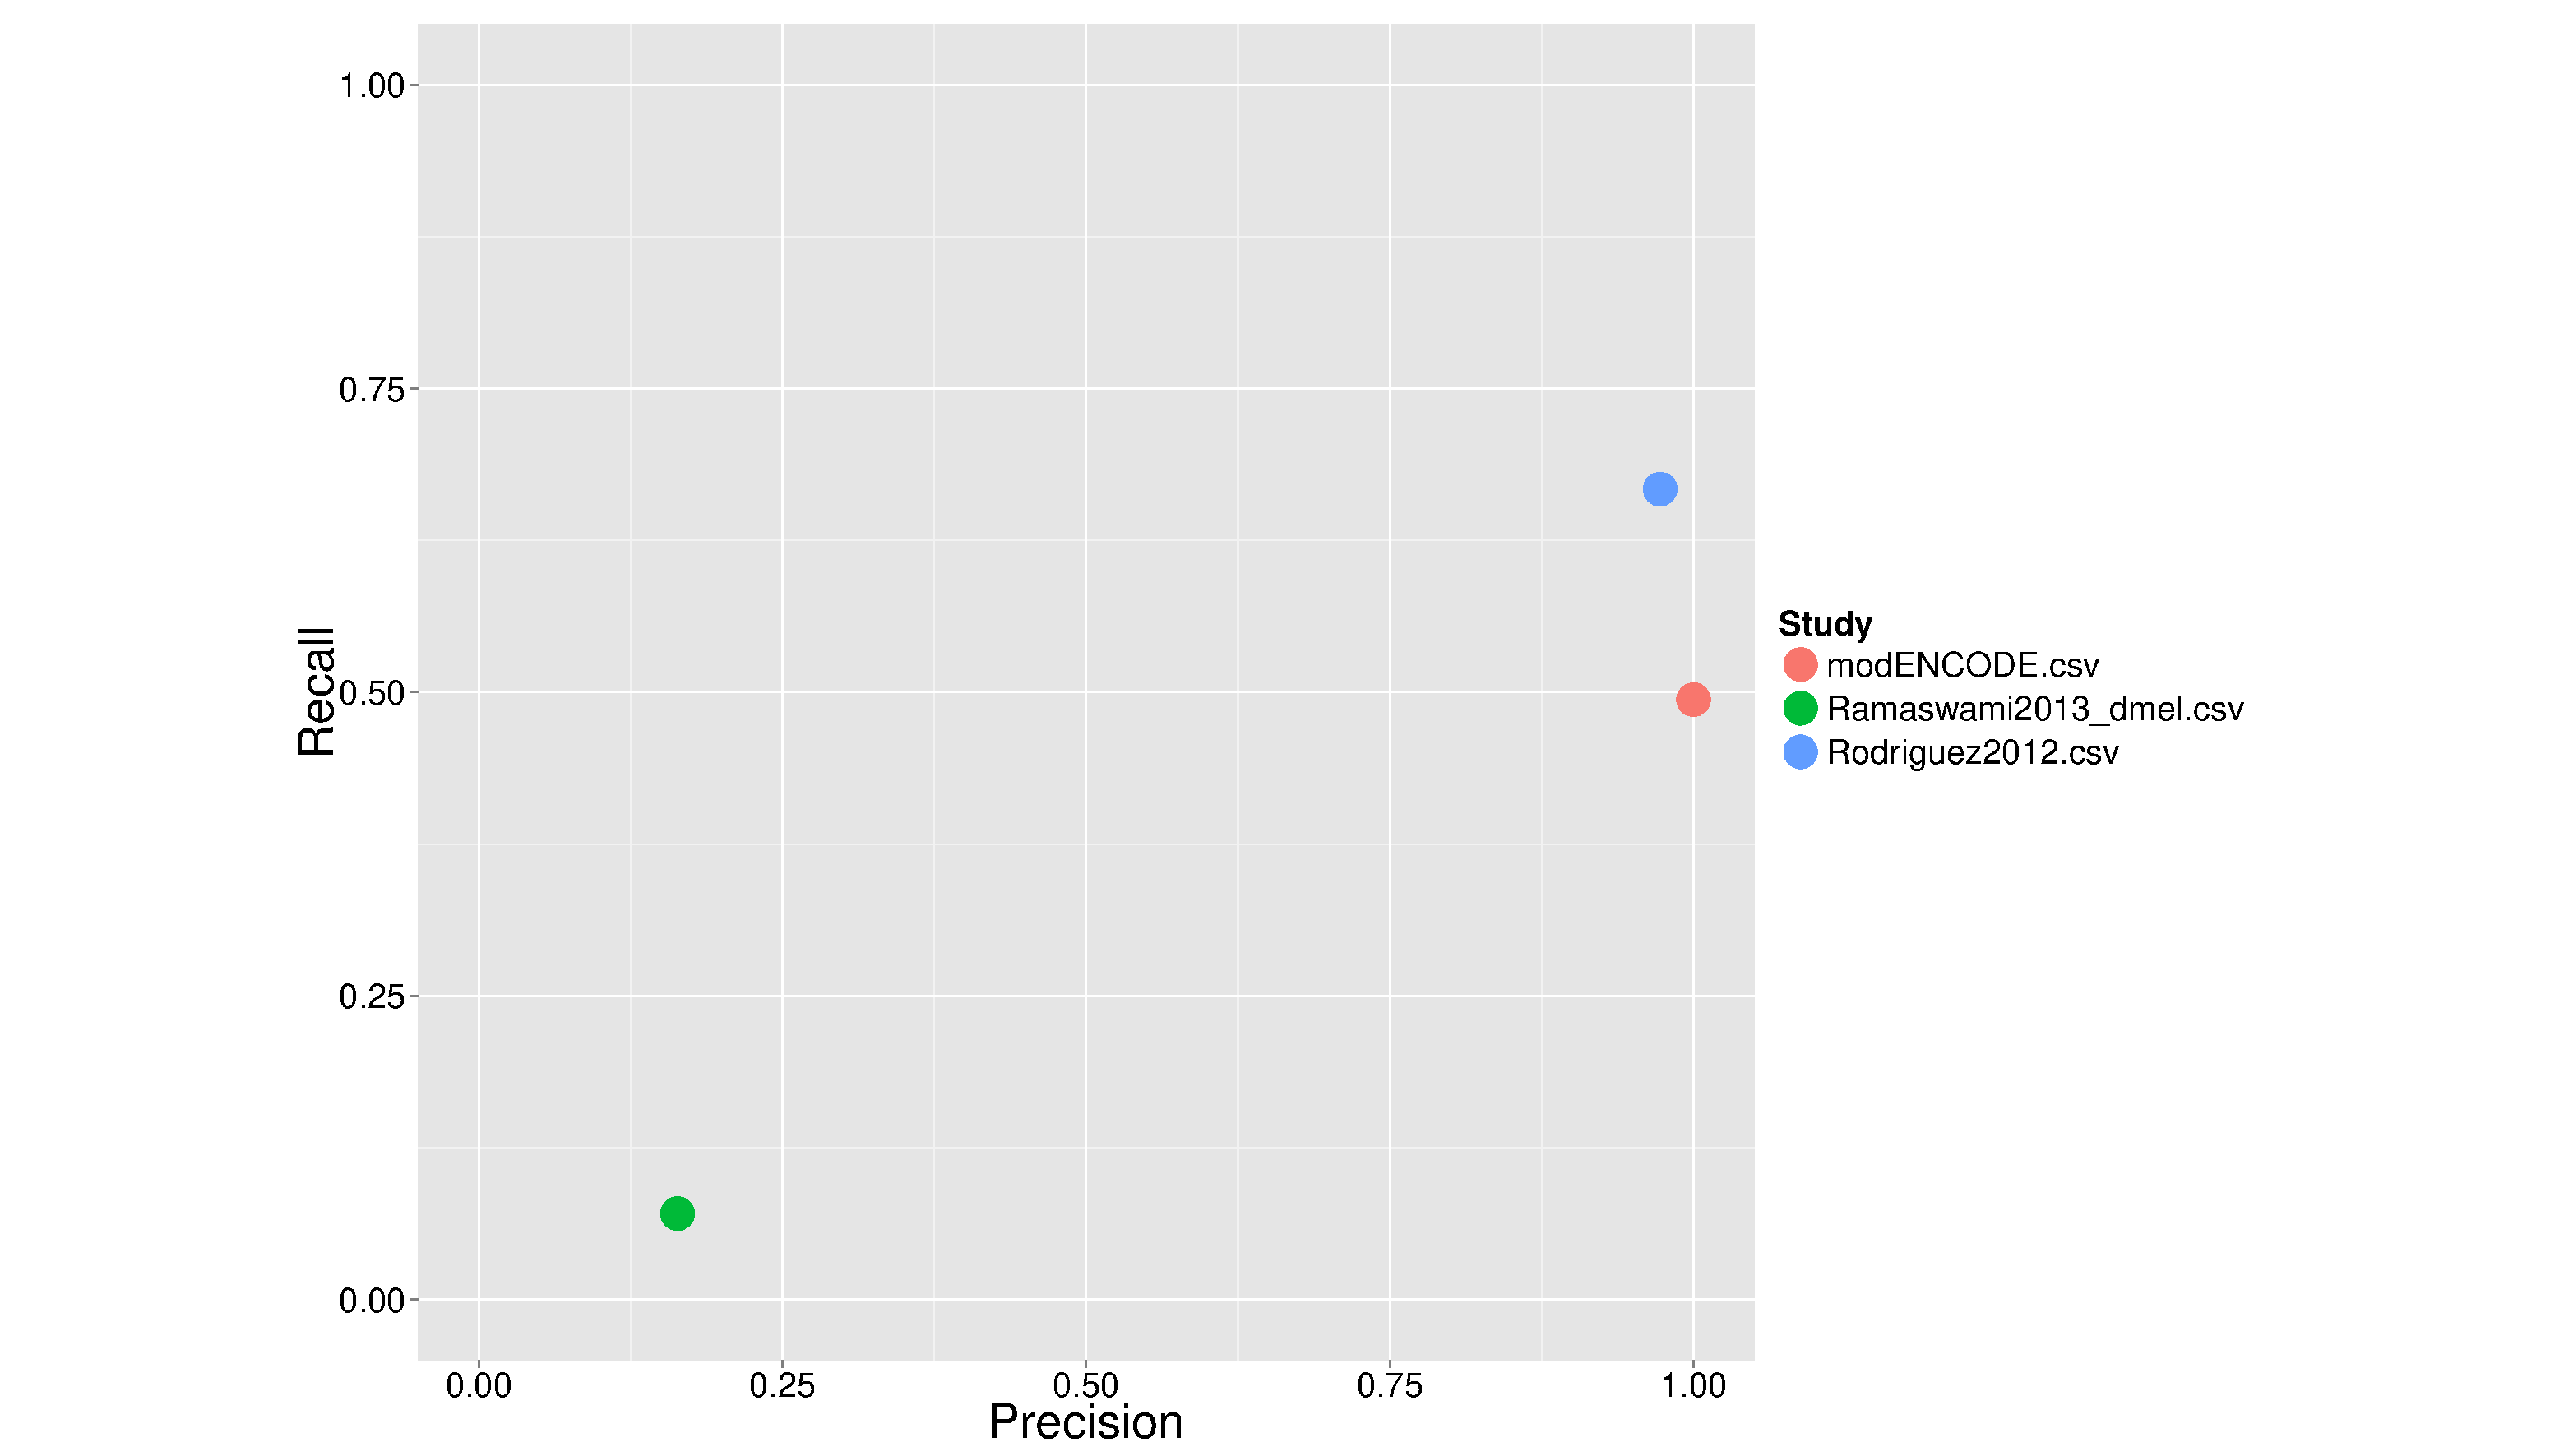
\includegraphics[width=14cm]{bench_fly.pdf}
	\end{center}
	\caption{ショウジョウバエのデータセットにおける適合率および再現率}
	\label{fig:fly_pr}
\end{figure}


\section{議論}
\subsection{高精度な検出手法の特徴}
\subsection{導入した指標の妥当性}
